\chapter{\IfLanguageName{dutch}{Schermafbeeldingen van het prototype}{Screenshots prototype}}%
\label{ch:screenshots-prototype}


\begin{center}
	\begin{figure}[H]
		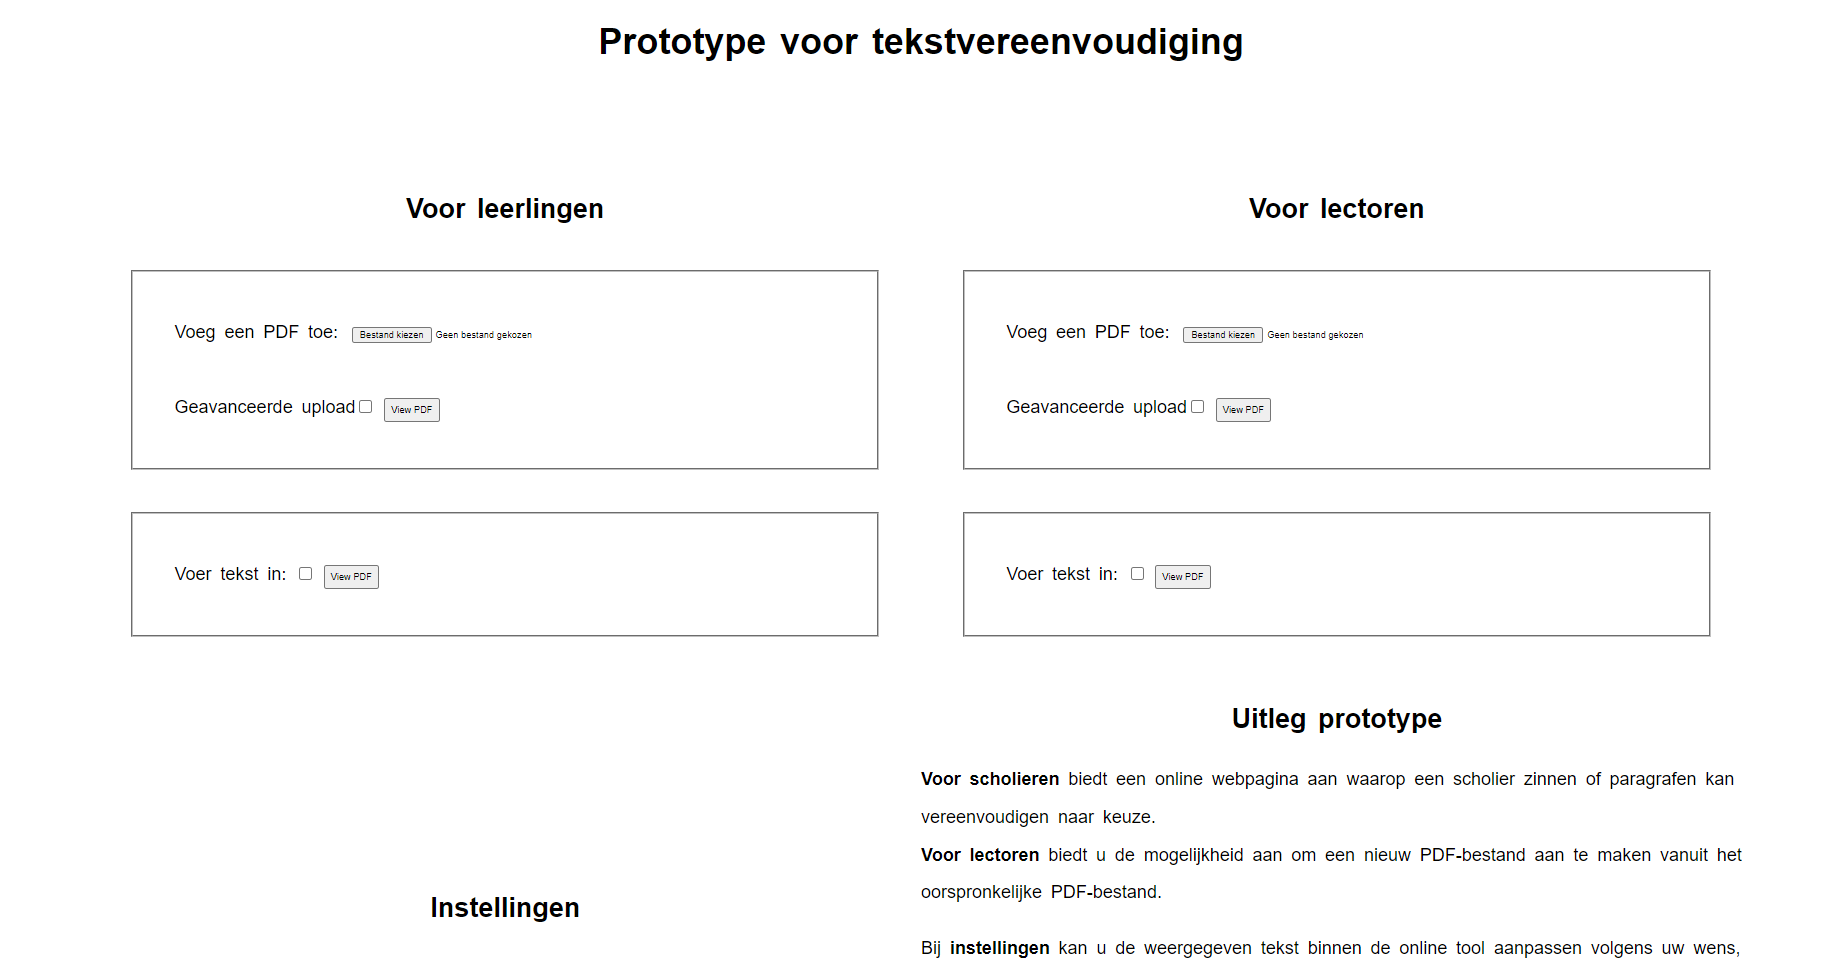
\includegraphics[width=\linewidth]{img/proto-homescreen.png}
		\caption{Een mogelijke weergaven van de homepagina.}		
		\label{img:homepage}
	\end{figure}
\end{center}

\begin{center}
	\begin{figure}[H]
		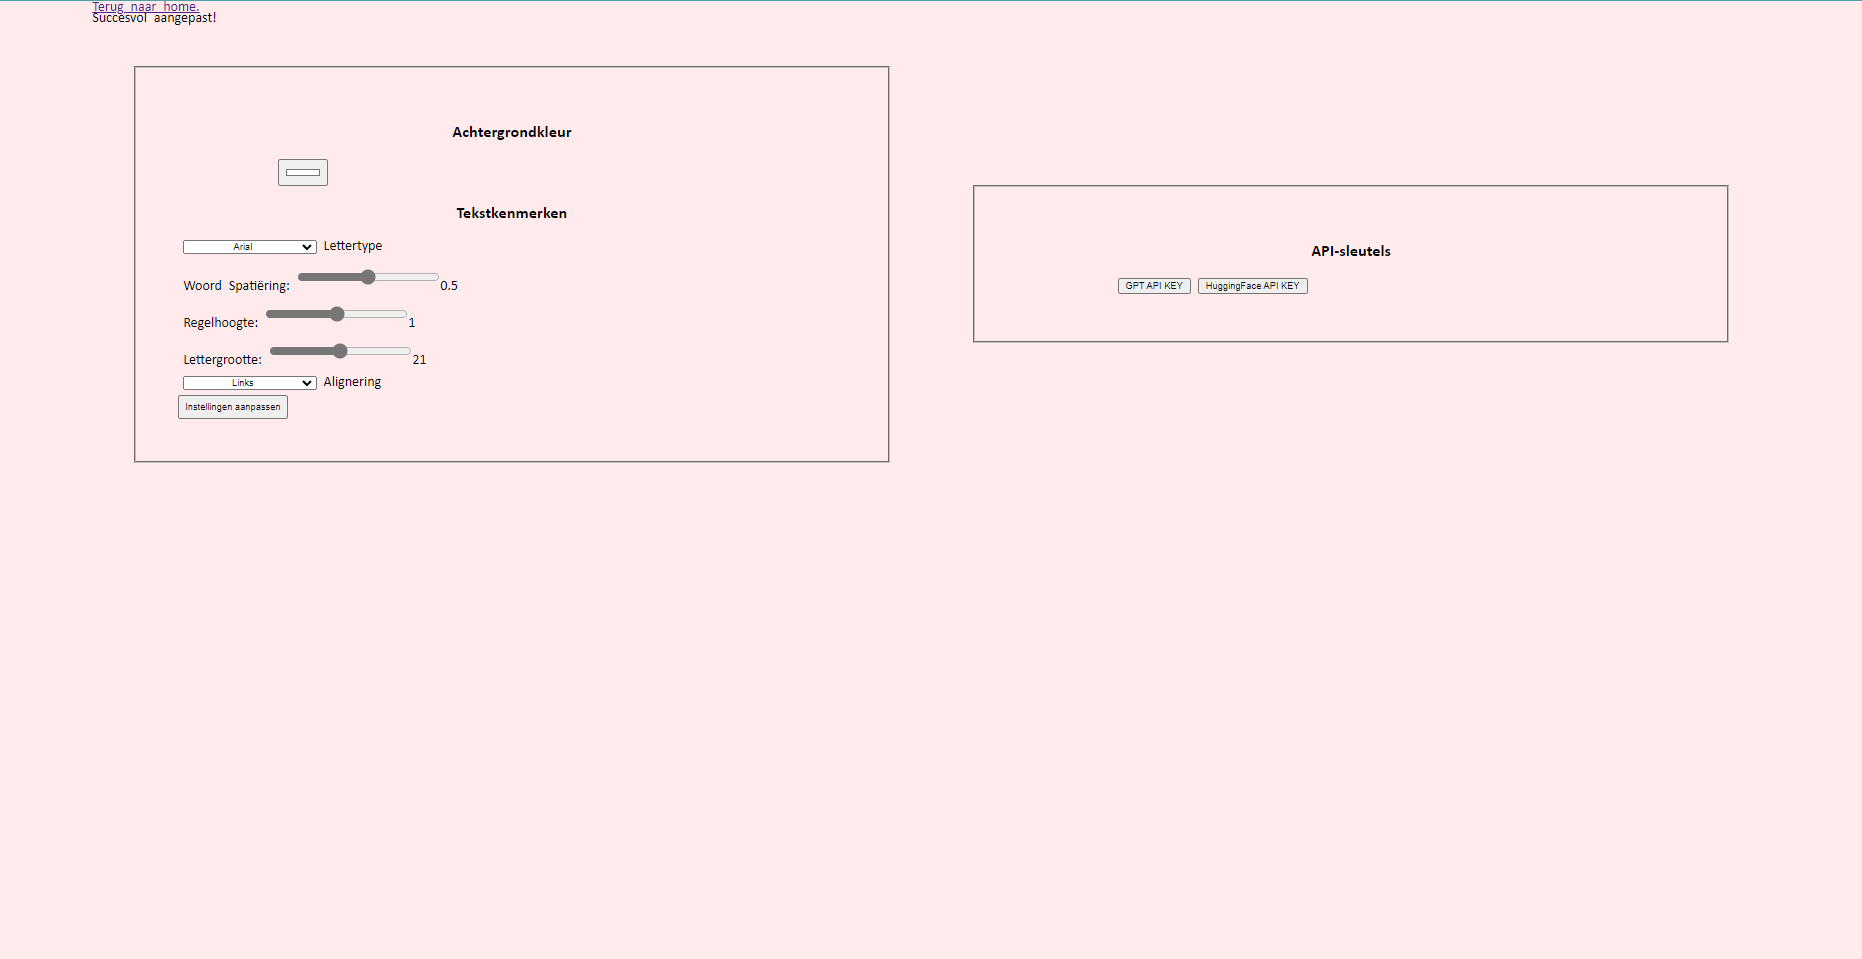
\includegraphics[width=\linewidth]{img/website-instellingen.png}
		\caption{Voorbeeldweergave van de instellingenpagina.}
		\label{img:website-instellingen}
	\end{figure}
\end{center}

\begin{figure}
	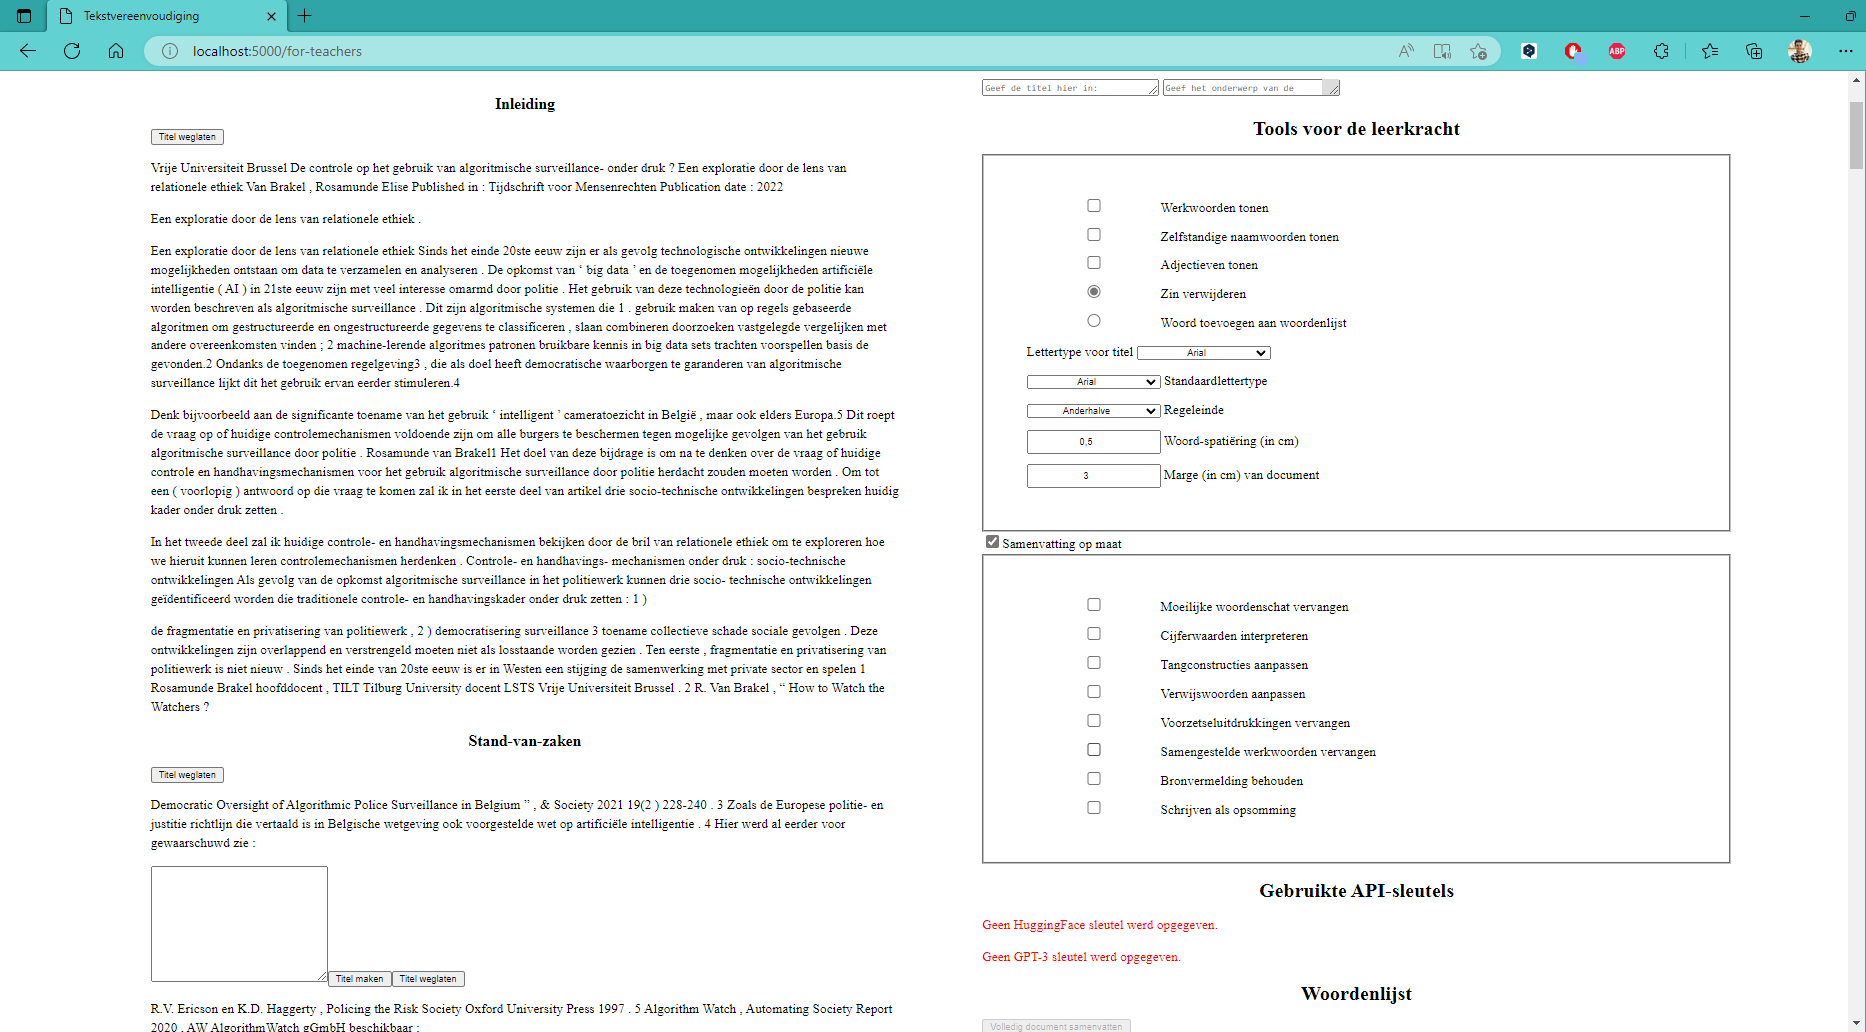
\includegraphics[width=\linewidth]{img/proto-lerarencomponent.png}
	\caption{Een mogelijke weergave van het lerarencomponent met het wetenschappelijk artikel van \textcite{VanBrakel2022} als input.}
	\label{img:proto-lerarencomponent}
\end{figure}

\begin{center}
	\begin{figure}[H]
		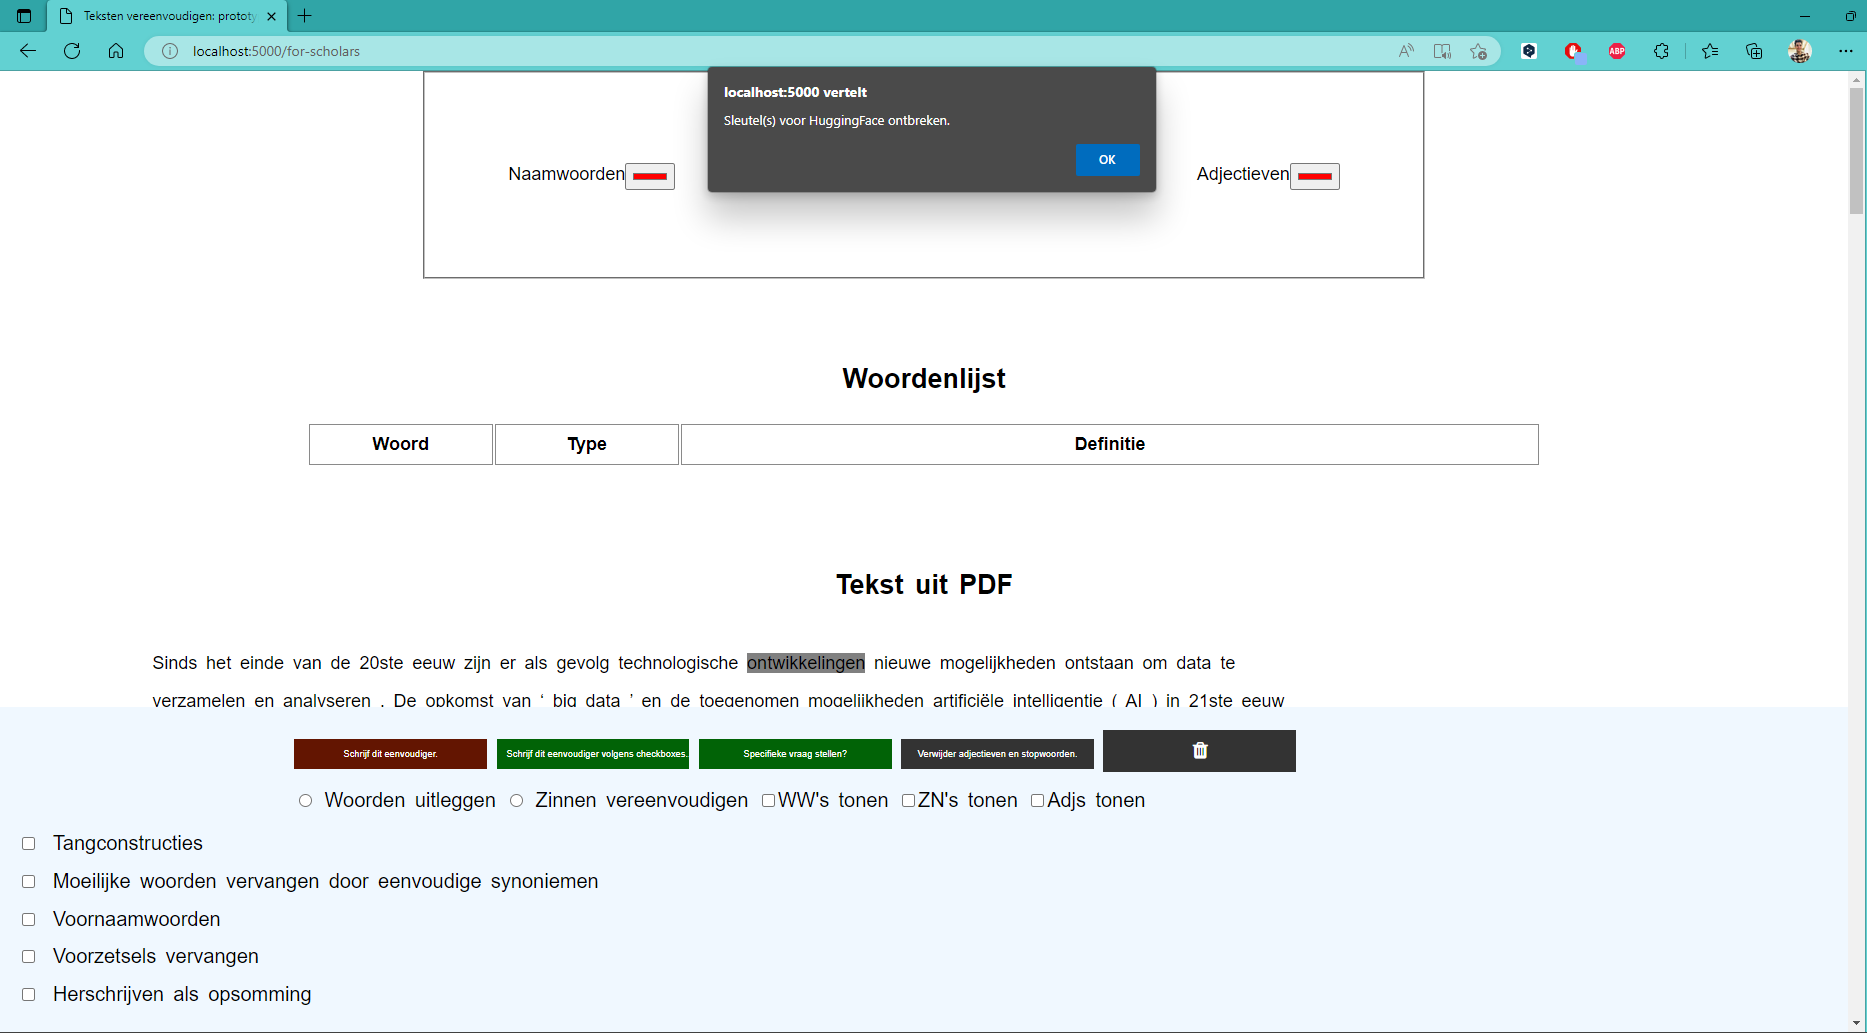
\includegraphics[width=\linewidth]{img/proto-melding.png}
		\caption{Een voorbeeldweergave van het scholierencomponent.}
		\label{img:proto-homescreen-scholieren}
	\end{figure}
\end{center}

\begin{center}
	\begin{figure}[H]
		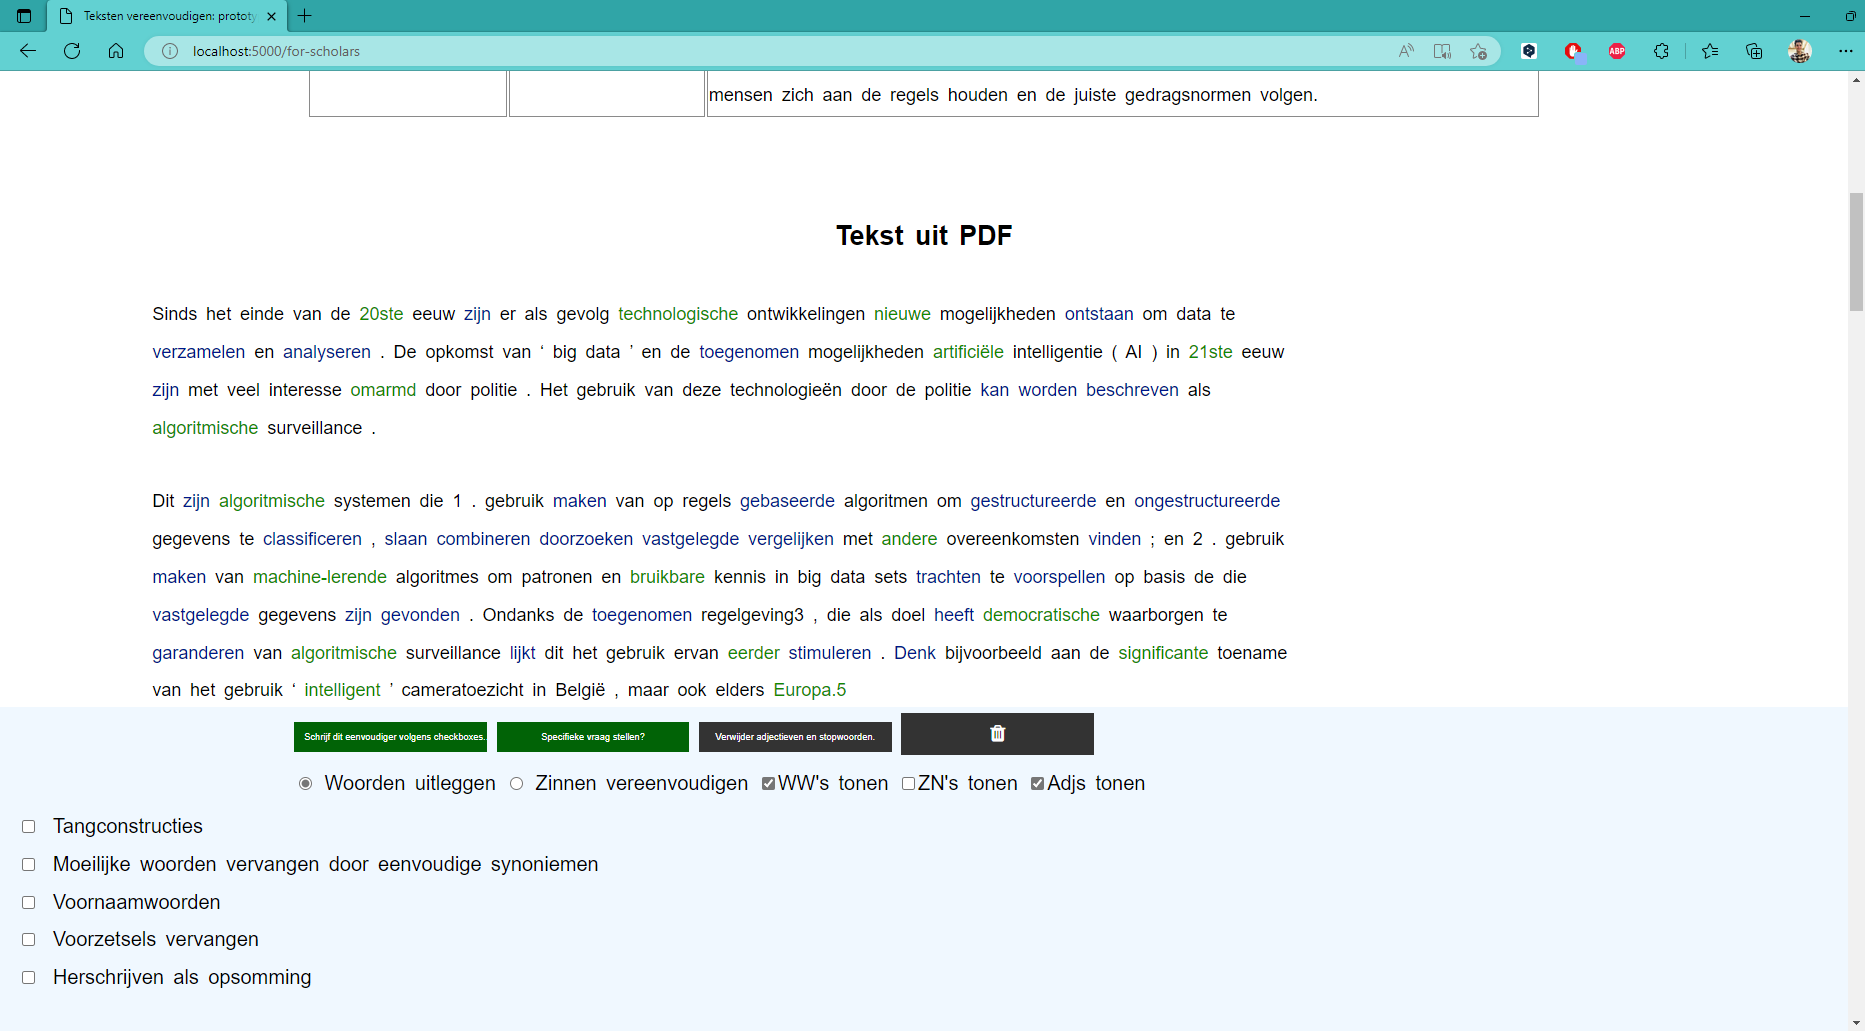
\includegraphics[width=\linewidth]{img/proto-pos-tagging.png}
		\caption{Een voorbeeldweergave van de toepassing van PoS-tagging bij het scholierencomponent.}
		\label{img:proto-pos-tagging-scholieren}
	\end{figure}
\end{center}

\begin{center}
	\begin{figure}[H]
		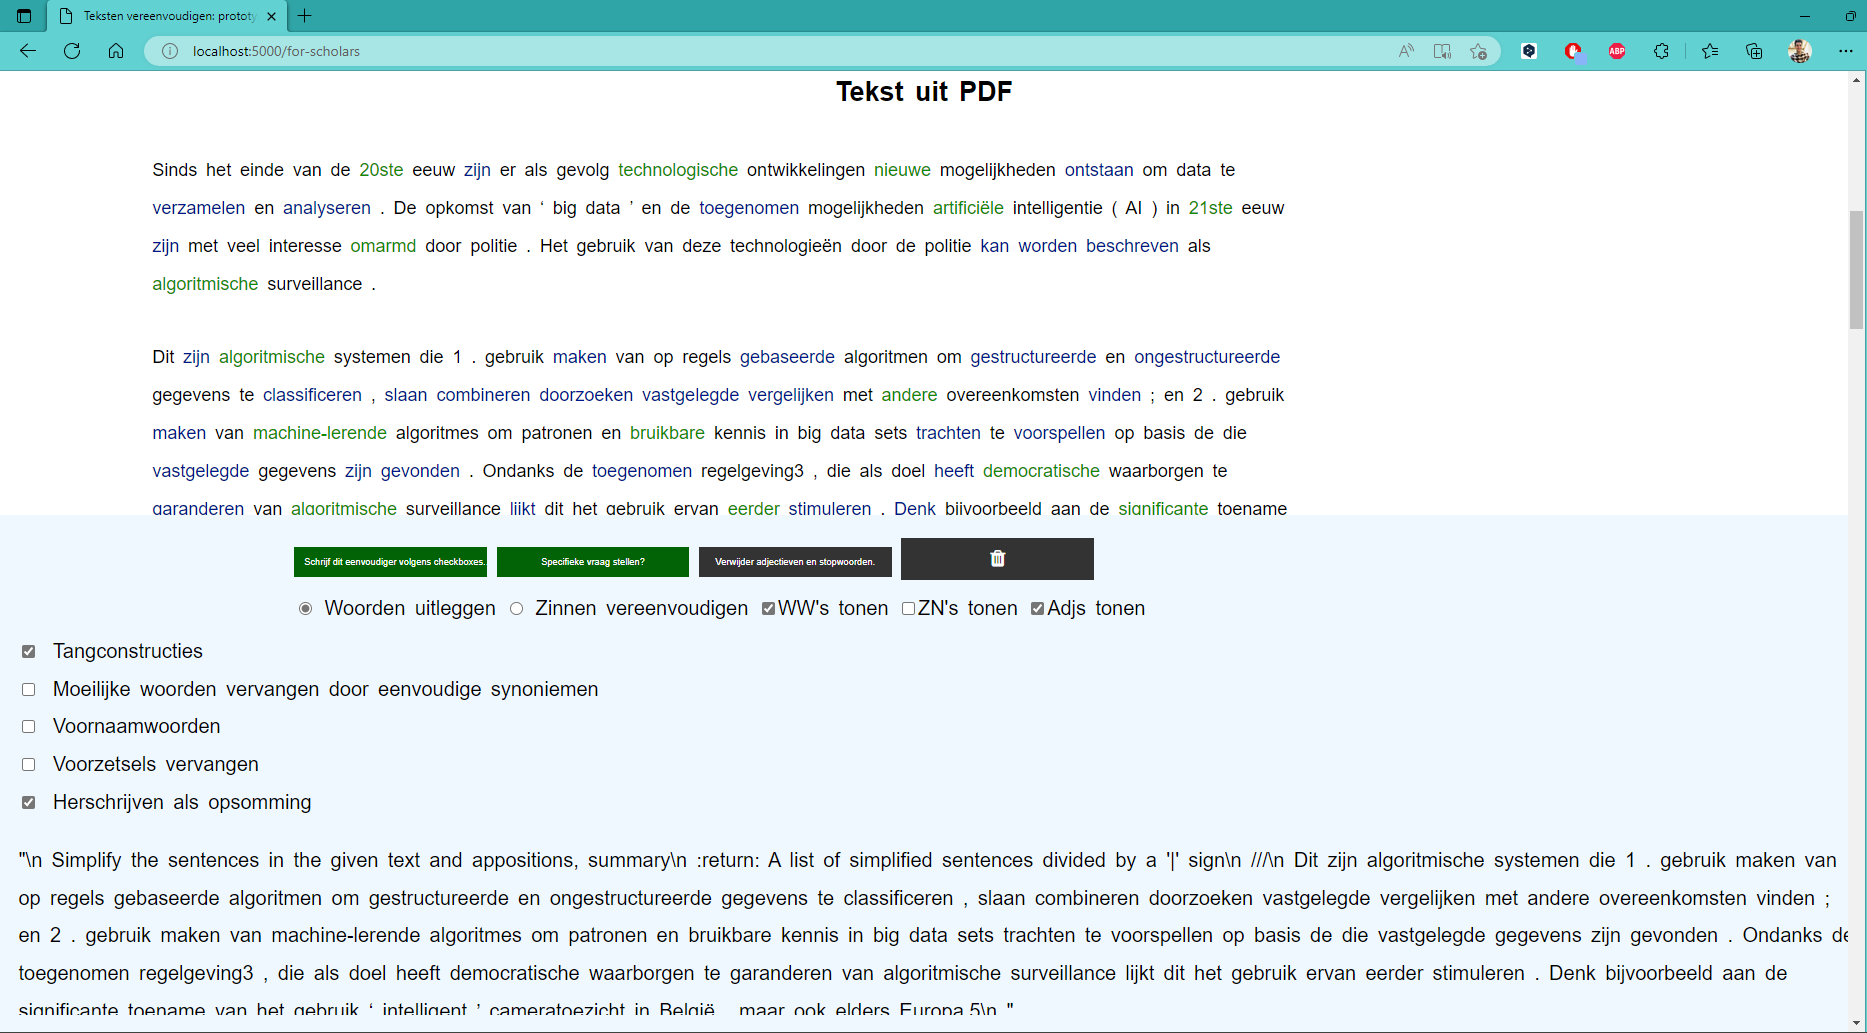
\includegraphics[width=\linewidth]{img/proto-opsomming-1.png}
		\caption{Stap 1 van een gepersonaliseerde tekstvereenvoudiging in het scholierencomponent.}
		\label{img:proto-scholieren-step-1}
	\end{figure}
\end{center}

\begin{center}
	\begin{figure}[H]
		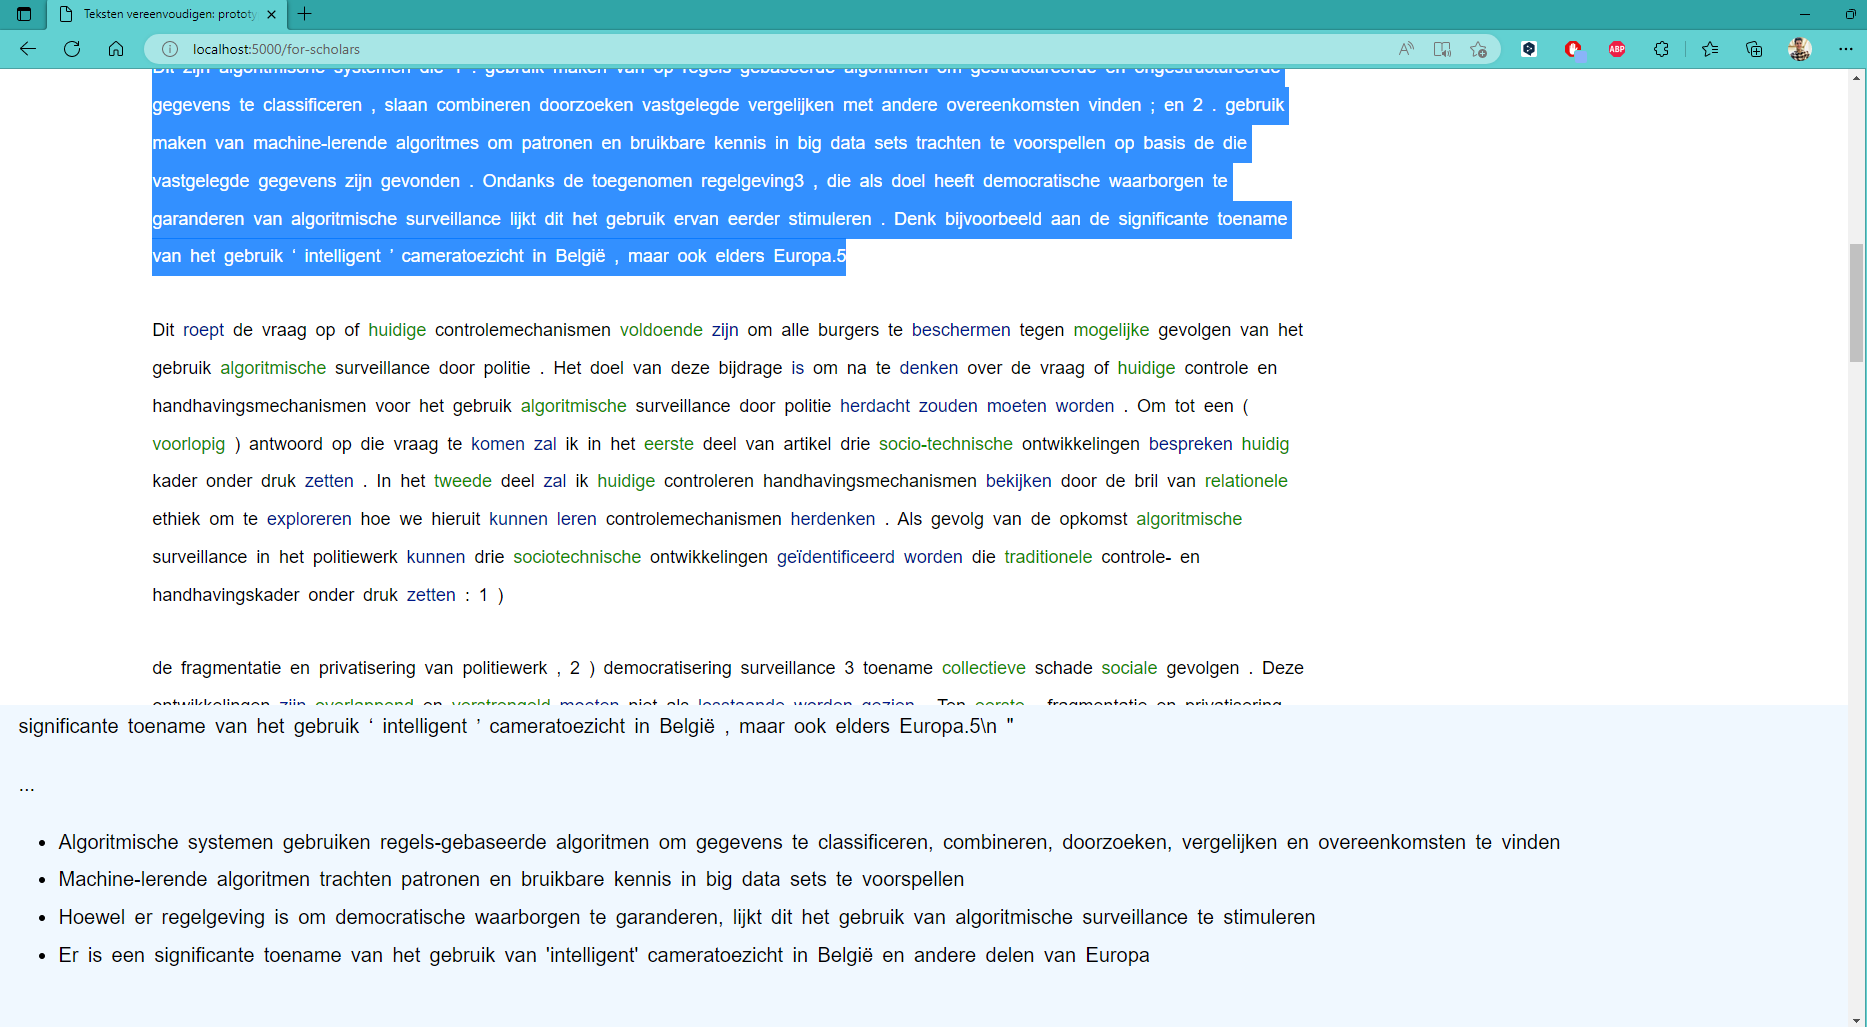
\includegraphics[width=\linewidth]{img/proto-opsomming-3.png}
		\caption{Stap 3 van een gepersonaliseerde tekstvereenvoudiging in het scholierencomponent.}
		\label{img:proto-scholieren-step-3}
	\end{figure}
\end{center}

\begin{center}
	\begin{figure}
		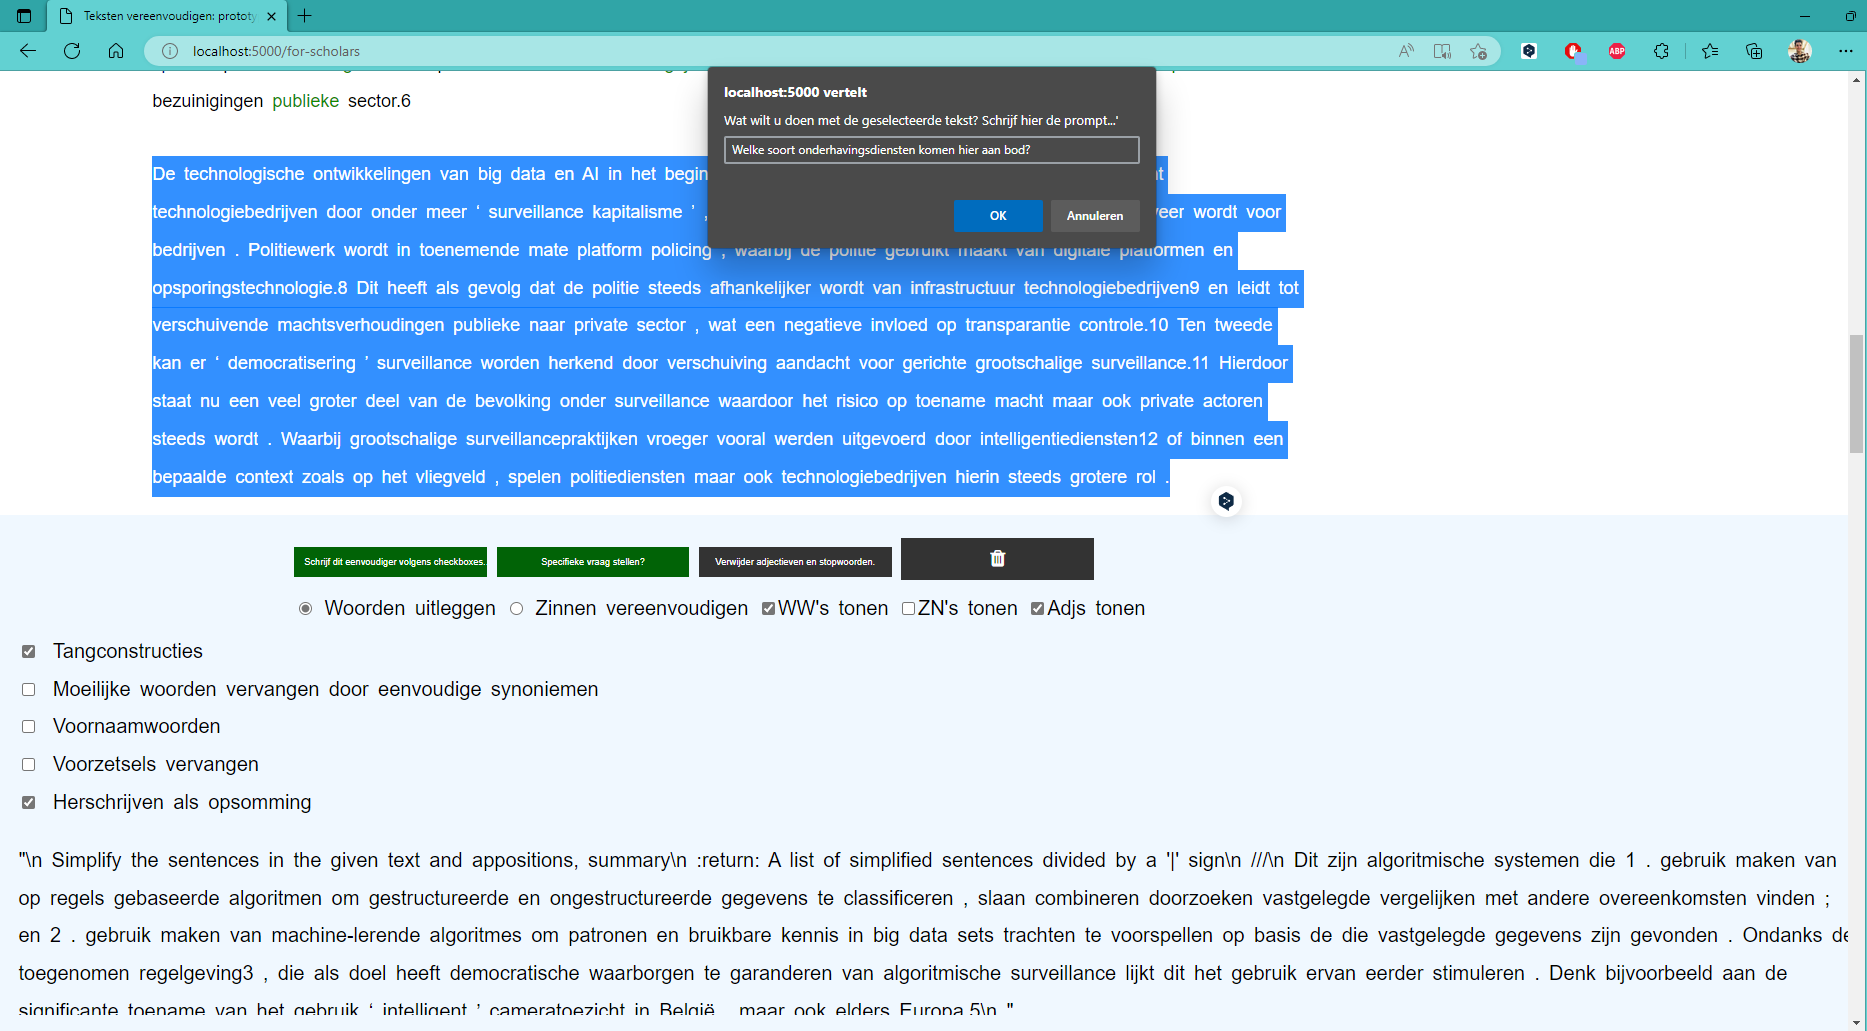
\includegraphics[width=\linewidth]{img/proto-vraagstelling-1.png}
		\caption{Stap 1 bij het stellen van een specifieke vraag bij gemarkeerde tekst.}
		\label{img:step-1-proto-vraagstelling}
	\end{figure}
\end{center}

\begin{center}
	\begin{figure}
		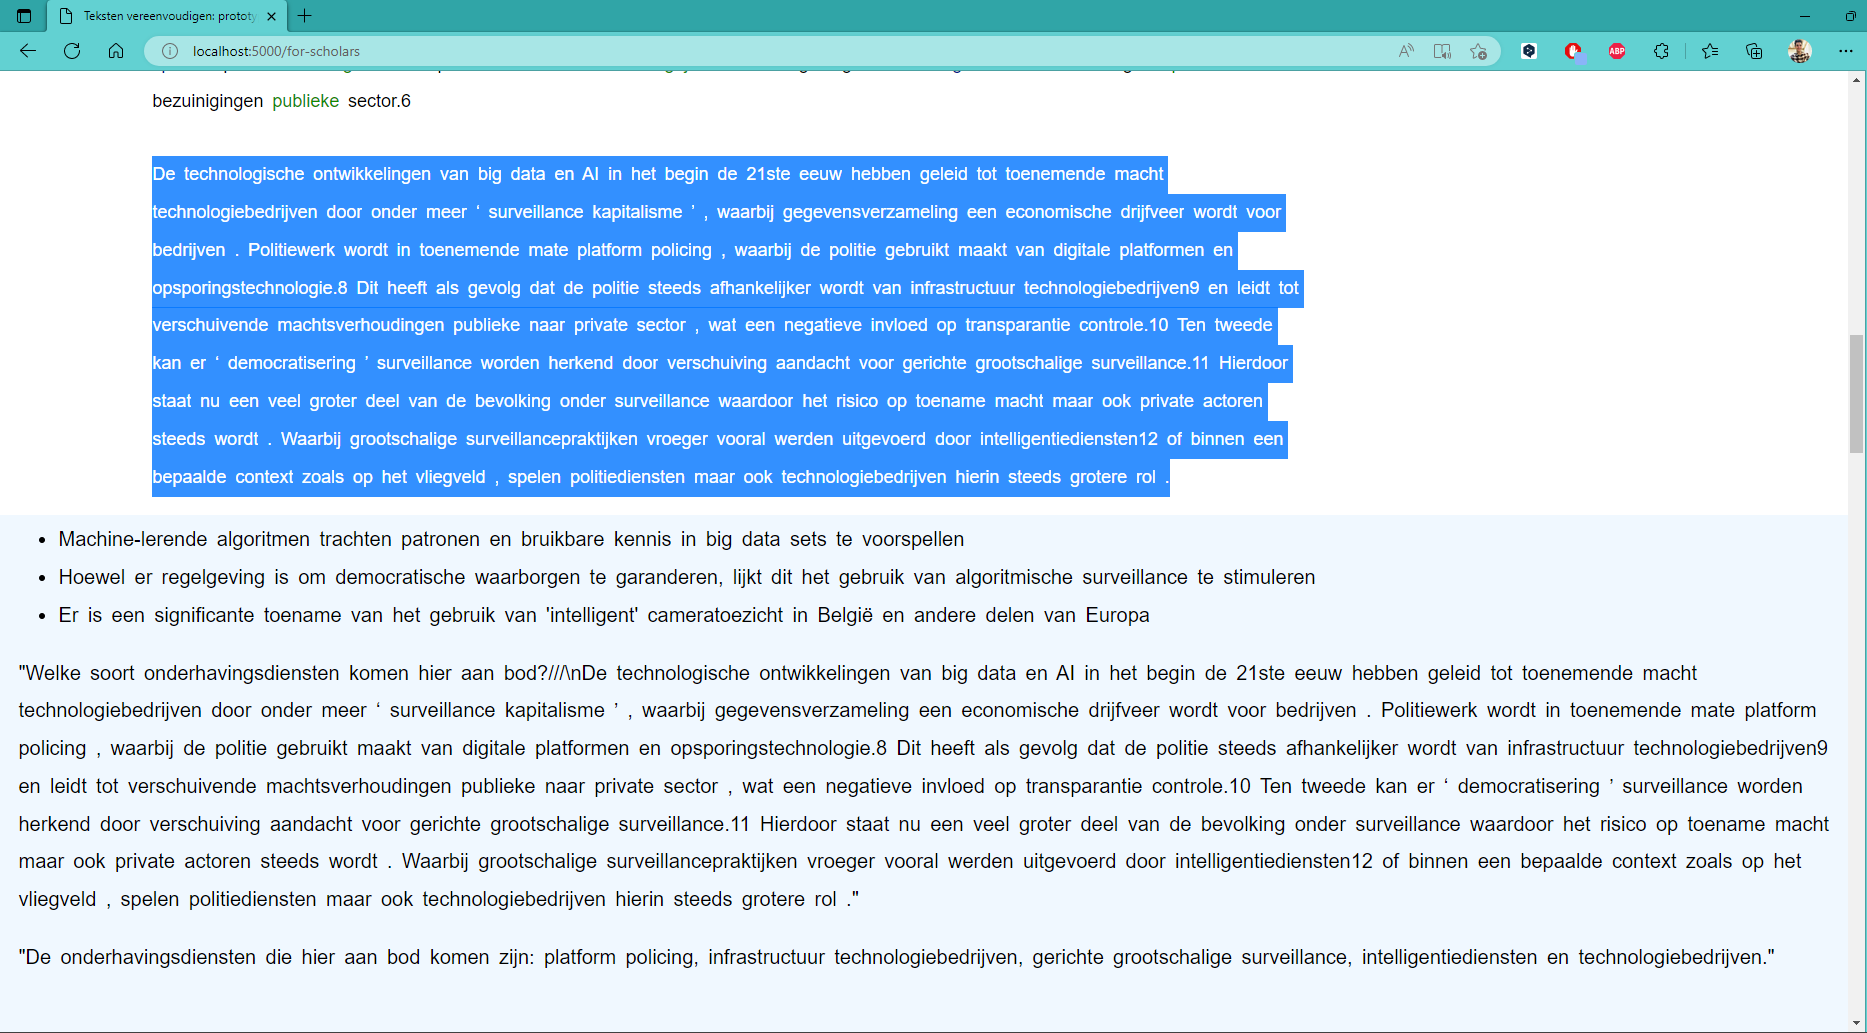
\includegraphics[width=\linewidth]{img/proto-vraagstelling-2.png}
		\caption{Stap 2 bij het stellen van een specifieke vraag bij gemarkeerde tekst.}
		\label{img:step-2-proto-vraagstelling}
	\end{figure}
\end{center}